% =====================================================================
%  Twin-in-the-Loop -- IEEE two-column conference manuscript
%  Status: DRAFT (2026-09-16).
%  Numbers: all gate, classifier, composition and statistics results are
%  from the CORRECTED simulator:
%    docs/research/uncertainty_and_gateway_ablation.md
%    docs/research/candidate_composition.md
%    docs/research/audit_fix1.md, docs/research/test_suite_audit.md
%  Figures measured only on the pre-correction simulator are labelled as
%  such in the text (latency, horizon sweep, fault-boundary split).
%  References are numbered in order of first citation.
% =====================================================================
\documentclass[conference]{IEEEtran}
\IEEEoverridecommandlockouts

\usepackage{cite}
\usepackage{amsmath,amssymb,amsfonts}
\usepackage{graphicx}
\usepackage{textcomp}
\usepackage{booktabs}
\usepackage{multirow}
\usepackage{tabularx}
\usepackage{array}
\usepackage{xcolor}
\usepackage{algorithm}
\usepackage{algpseudocode}
\usepackage{tikz}
\usetikzlibrary{arrows.meta,positioning,shapes.geometric,shapes.misc,calc,patterns}
\usepackage{pgfplots}
\pgfplotsset{compat=1.17}
\usepackage[hidelinks]{hyperref}

\renewcommand{\arraystretch}{1.12}
\newcolumntype{Y}{>{\raggedright\arraybackslash}X}

\begin{document}

\title{Twin-in-the-Loop: Separating Prediction from Blocking When a Digital Twin Vets Autonomous Edge-Network Repairs}

\author{
\IEEEauthorblockN{
Nitin Kumar Pandey\IEEEauthorrefmark{1},
Ayush Raj\IEEEauthorrefmark{1},
Abhay Mahantesh Zalaki\IEEEauthorrefmark{1},
Guneet Kaur Arora\IEEEauthorrefmark{1},
Syamasudha Veeragandham\IEEEauthorrefmark{1}
}

\IEEEauthorblockA{\IEEEauthorrefmark{1}School of Computer Science and Engineering,
Vellore Institute of Technology, Vellore, India\\
\{nitinkumar.pandey2023, ayush.raj2023a, abhay.mahantesh2023, guneetkaur.arora2023\}@vitstudent.ac.in,
syamsudha.v@vit.ac.in}
}

\maketitle

% =====================================================================
\begin{abstract}
Autonomous controllers, including agents built on large language models, are increasingly proposed as operators for edge and IoT networks. A common safeguard executes each proposed repair on a digital twin and applies it only if the predicted outcome is acceptable. Such gates are usually evaluated against an ungated agent, which cannot separate the value of the twin's predictions from the value of blocking. We present Twin-in-the-Loop, an open testbed that places a validation gate between a controller and a deterministic, forkable 17-node edge-network simulator with six composable fault types. The twin is degraded along five configurable axes controlled by one fidelity scalar and is rolled forward without access to the fault schedule. Every proposal, including rejected ones, receives a paired counterfactual harm label, so the gate can be scored both as a classifier and by closed-loop service-level-objective (SLO) violations. Rule-based and scripted aggressive controllers are compared under ungated, reject-all, random, twin, and schedule-aware gates over ten paired seeds, with exact Wilcoxon tests and Holm correction. At full fidelity the twin is a near-perfect local filter: it preserves 100\% of available benefit and prevents 100\% of available harm for the rule controller, and 92.9\% and 97.6\% for the scripted controller. Yet it cannot be distinguished from reject-all at the episode level. The rule controller's 4.4 violation-tick advantage comes from a single seed (exact $p = 1.000$). The only effects that survive correction are that the scripted controller is harmful when ungated and that any blocking gate removes about 30 violation-ticks of that harm (Holm $p = 0.0215$). Candidate-composition analysis explains the null: reject-all discards only 35 and 2 violation-ticks of benefit across ten episodes, so even a perfect gate would have about 17\% power. A gateway ablation rules out a topology artifact. Gate evaluations should report reject-all controls and available benefit alongside classifier accuracy.
\end{abstract}

\begin{IEEEkeywords}
Digital twin, edge networks, autonomous remediation, safety gate, counterfactual evaluation, LLM agents, service-level objectives, reject-all ablation
\end{IEEEkeywords}

% =====================================================================
\section{Introduction}

\textbf{Background: autonomous operation of networked services.} Operating edge and IoT networks under faults such as saturated nodes, crashed devices, degraded links, memory leaks, and traffic surges requires remediation decisions faster than human operators can make them. These decisions are increasingly delegated to automated controllers and, more recently, to agents driven by large language models (LLMs). Benchmarks now evaluate such agents on microservice remediation~\cite{microremed}, network troubleshooting~\cite{nika}, and stateful network configuration~\cite{netagentbench}, which shows that autonomous operation is an active research target rather than a distant prospect.

\textbf{Digital twins as a pre-actuation safeguard.} A wrong action applied to a live network can cause lasting damage, so a recurring design places a digital twin between the decision maker and the network. The proposed change is first executed on the twin, and only changes predicted to be acceptable are applied. Aether coordinates network-operations agents with a network digital twin to validate configuration changes on an ISP laboratory replica~\cite{aether}, and recent process-plant work lets an LLM agent propose actions that are validated in simulation and re-prompted on failure~\cite{processplant}. The twin-gated pattern is therefore established; what is less established is how to measure what the twin contributes.

\textbf{Lineage in safety-critical control.} The idea of checking an advanced controller's output against a model before actuation predates LLMs. The Simplex architecture separates a high-performance controller from a simple verified safety controller that takes over before failure~\cite{simplex}. Predictive safety filters forward-simulate a proposed input and minimally modify it when it cannot be certified~\cite{wabersich}, and model predictive shielding uses forward simulation to decide whether a learned policy may act or must hand control to a backup policy~\cite{mps}. Finite-horizon prediction, terminal conditions, and robustness to model error are treated systematically in model predictive control~\cite{rawlings}. Our gate is a deliberately simple member of this family.

\textbf{Motivation: outcome improvement does not measure prediction.} Evaluating a twin gate is harder than building one. Real networks cannot be replayed, so the true consequence of a \emph{rejected} change is rarely observed, and evaluations tend to report outcome improvement over an ungated agent. That comparison conflates two sources of benefit: the gate's ability to tell good actions from bad ones, and the simple fact that it blocks something. If most of an agent's proposals are harmful, a gate that blocks everything looks excellent while predicting nothing. NetInjectBench makes this concrete for tool-using network agents by showing that a static allowlist reduces unsafe actions but destroys the usefulness of approved changes~\cite{netinjectbench}.

\textbf{Motivation: safety must be reported with utility.} Security evaluations of agents have converged on reporting utility and attack success together, because either number alone can be optimised trivially. AgentDojo reports utility, utility under attack, and attack success side by side and cautions against reducing them to a single leaderboard~\cite{agentdojo}. The analogous requirement for twin gates is that harm prevented must be reported together with benefit preserved, and both must be compared with a no-prediction control.

\textbf{Motivation: twins are never exact.} Any deployed twin differs from the system it models through observation noise, stale state, drifting parameters, forecast error, and simplified dynamics. Monotone gains with fidelity should not be assumed: in additive manufacturing, lower-fidelity twins can detect failures comparably to higher-fidelity ones~\cite{fidelityam}. Model-based reinforcement learning likewise studies how prediction length trades usefulness against compounding model bias~\cite{mbpo}. Fidelity is rarely varied systematically in agentic network settings, which motivates a controllable-fidelity twin.

\textbf{Motivation: faults are only partially observable.} A controller sees symptoms, not causes, and a twin rolled forward from the current state cannot know which faults will arrive in the future. Whether a fault can be inferred from observed behaviour is a question of diagnosability that is distinct from state observability~\cite{sampath}, and planning under partial observability typically relies on sampling hidden states through a black-box simulator~\cite{pomcp}. We make this limitation explicit by rolling the twin forward \emph{fault-blind} and comparing it with a gate that can see the schedule.

\textbf{Motivation: operational repair semantics matter.} Real repair actions have costs and interact. Production orchestrators implement reconciling control loops that drive observed state toward desired state~\cite{k8scontroller}, autoscalers use tolerances and stabilisation windows to avoid oscillation~\cite{k8shpa}, and site-reliability practice documents how a failed replica can push load onto the survivors and trigger a cascade~\cite{sre_cascade}. A testbed that treats restarts and migrations as free would overstate the value of acting, so our simulator charges explicit downtime and drops.

\textbf{Motivation: bounded agents need bounded evaluation.} Agent loops are bounded by step or tool budgets, and behaviour at the bound affects outcomes. Budget-aware tool use shows that exposing the remaining budget changes how agents scale~\cite{budgetaware}, and graph-based agent frameworks raise explicit errors when recursion limits are reached~\cite{langgraph}. Our controllers operate under a bounded retry budget with a no-op fallback, so the gate's rejection behaviour and the controller's retry behaviour must be analysed together.

\textbf{Scope: a measurement instrument, not a new safety guarantee.} Using common random numbers to compare alternatives in simulation is standard~\cite{crn}, and it has recently been applied to rollout-based planning, where the continuation policy affects the variance of relative utilities~\cite{yadav}. Action-level safety labels and shields have been formalised with explicit false positives and negatives~\cite{rulebasedshield}, and safe and constrained reinforcement learning has been surveyed extensively~\cite{saferlsurvey}. We do not claim that twin-gated validation, paired simulation, or shielding is new. The contribution is a testbed and protocol that isolate what the twin's \emph{prediction} adds, run on a synthetic simulator whose limits are stated in Section~\ref{sec:limits}.

\textbf{Contributions.} The paper makes four contributions. (i) A deterministic, forkable edge-network simulator with six composable fault types, a closed six-action repair schema with three-layer validation, and a streaming telemetry chain. (ii) A twin gate degraded along five independent axes and rolled forward without the fault schedule. (iii) A paired counterfactual protocol that scores the gate as a classifier and in closed loop against reject-all, random, and schedule-aware controls, with exact tests and multiplicity correction. (iv) Empirical evidence that an accurate local filter need not yield a detectable episode-level advantage, together with a candidate-composition analysis that explains why.

\subsection{Research Objectives}

\begin{enumerate}
  \renewcommand{\labelenumi}{\textbf{RO\arabic{enumi}.}}
  \item To design a deterministic, forkable edge-network testbed in which a digital-twin gate of controllable fidelity vets repair proposals from interchangeable controllers.
  \item To define a paired counterfactual evaluation protocol that labels every proposal, including rejected ones, and scores the gate both as a harm classifier and by closed-loop SLO violations.
  \item To determine, with exact paired statistics, whether a twin gate improves outcomes beyond no-prediction controls (reject-all and random gating) and beyond a schedule-aware gate.
  \item To explain the relationship between local classifier quality and episode-level benefit through candidate composition, and to test whether an unfaultable gateway node biases the results.
\end{enumerate}

% =====================================================================
\section{Related Work}

\textbf{Digital twins for network change validation.} Aether coordinates five network-operations agents with a network digital twin to validate configuration changes on a 25-router ISP laboratory replica~\cite{aether}. It reports 94\% error detection with 0.64 precision on synthetic scenarios and 100\% detection on two past incidents, while final deployment approval remains with a human. It does not sweep twin fidelity or report a reject-all control. Our work is complementary: a far simpler network, but a protocol that isolates prediction from blocking.

\textbf{LLM agents with simulation-in-the-loop fault handling.} The process-plant study of~\cite{processplant} is the closest propose--simulate--validate--reprompt architecture. It reports correct, incorrect, and missed actions and reprompt counts across models and input representations for a clogging scenario. Its agent has access to state and fault type, and after retries are exhausted it forces the action. Our controllers see symptoms only, and our fallback after rejection is a no-op, which changes what a rejection costs.

\textbf{Remediation benchmarks for services.} MicroRemed benchmarks LLMs that generate remediation playbooks for microservice failures and evaluates recovery~\cite{microremed}. SLBench evaluates skill-following and mitigation behaviour and reports a reduction in violations on a selected set of previously violating cases~\cite{slbench}. These benchmarks measure the proposer; neither isolates the contribution of a model-based validation gate.

\textbf{Network troubleshooting and configuration benchmarks.} NIKA provides an arena for benchmarking agents on realistic network diagnosis and localisation~\cite{nika}, and NetAgentBench evaluates stateful, multi-turn network configuration~\cite{netagentbench}. They supply richer network semantics than our simulator but no counterfactual label for rejected actions, which is the quantity our protocol is built around.

\textbf{Safety versus utility for tool-using agents.} NetInjectBench reports unsafe tool-action rates for network agents under indirect prompt injection and shows that a static allowlist achieves safety at the cost of approved-change usefulness~\cite{netinjectbench}. AgentDojo reports utility and attack success jointly~\cite{agentdojo}. Our reject-all ablation applies the same principle to a closed-loop network setting: a gate that never approves anything is the baseline that prediction must beat.

\textbf{Predictive safety filters and shielding.} Simplex~\cite{simplex}, predictive safety filters~\cite{wabersich}, and model predictive shielding~\cite{mps} forward-simulate a proposed action and fall back to a backup policy. Robust model predictive shielding extends the idea to stochastic disturbances with sampled trajectories~\cite{robustmps}. These methods provide recoverability guarantees under model assumptions; our gate provides none. It approves an action if predicted violations over a finite horizon are no worse than those of a no-op.

\textbf{Shields and safe reinforcement learning.} Rule-based shields define ground-truth safety labels on state--action pairs and discuss false positives and negatives of a binary shield~\cite{rulebasedshield}. A recent survey maps safe and constrained reinforcement learning across single- and multi-agent settings~\cite{saferlsurvey}. We borrow the classifier view of a shield but add closed-loop episode outcomes and no-prediction controls, since classifier accuracy alone does not establish operational value.

\textbf{Model fidelity and decision-aware modelling.} Su \emph{et al.} vary six digital-twin attributes for material-extrusion failure detection and find that lower-fidelity twins can perform comparably~\cite{fidelityam}. MBPO studies the tradeoff between rollout length and model bias~\cite{mbpo}, and value-aware model learning weights model error by its effect on decisions~\cite{vaml}. Both lines suggest that the relevant question is not how accurate a twin is but whether its errors change decisions, which our fidelity sweep and composition analysis test directly.

\textbf{Common random numbers and paired simulation.} Common random numbers reduce the variance of differences between simulated alternatives~\cite{crn}. Yadav \emph{et al.} use them for simulation-based planning with rollouts and show that the continuation policy affects relative-utility variance~\cite{yadav}. Our paired action/no-op forks implement this established technique; they are not a new causal method, and our labels inherit the no-op continuation assumption.

\textbf{Diagnosability and planning under partial observability.} Diagnosability asks whether observed behaviour can establish that a fault occurred~\cite{sampath}, a question extended to labelled Petri nets~\cite{cabasino}. POMCP plans with a black-box simulator by sampling hidden states from a belief~\cite{pomcp}. Our fault-blind twin sits at the simplest end of this space: it assumes current faults persist and future faults do not occur, and a schedule-aware gate quantifies the cost of that assumption.

\textbf{Operational control loops and observability practice.} Kubernetes controllers reconcile observed and desired state~\cite{k8scontroller}, and the HorizontalPodAutoscaler uses metric ratios, tolerances, and stabilisation windows~\cite{k8shpa}. Site-reliability guidance on monitoring distinguishes symptoms from causes~\cite{sre_monitoring} and describes cascading overload~\cite{sre_cascade}. These practices inform our action costs and SLO definitions, but production systems rarely log counterfactual outcomes of rejected changes, which is why a deterministic testbed is useful.

\begin{table*}[t]
\centering
\caption{Representative prior works and their relationship to this work.}
\label{tab:related}
\small
\begin{tabularx}{\textwidth}{@{}p{2.6cm}p{2.5cm}YYY@{}}
\toprule
Work & Domain & Validation / safety mechanism & Evaluation controls reported & Relationship to this work \\
\midrule
Aether~\cite{aether} & ISP network change validation & Network digital twin with agents; human approval & Detection rate, precision on synthetic and historical incidents & Same pattern; we add fidelity sweep and reject-all control \\
Process plant~\cite{processplant} & Industrial process control & Simulation validation with LLM re-prompting & Correct / incorrect / missed actions, reprompts & Closest loop; our agents see symptoms only and fall back to no-op \\
MicroRemed~\cite{microremed} & Microservices & None (proposer benchmark) & Recovery success & Measures proposer; we measure the gate \\
NIKA~\cite{nika}, NetAgentBench~\cite{netagentbench} & Network troubleshooting, configuration & None (proposer benchmark) & Diagnosis and configuration correctness & Richer networks; no counterfactual labels \\
NetInjectBench~\cite{netinjectbench} & Network agent security & Allowlist and defences & Unsafe-action rate with utility & Same safety--utility principle, open-loop \\
Predictive safety filter~\cite{wabersich}, MPS~\cite{mps} & Continuous control & Forward simulation with backup policy & Constraint satisfaction guarantees & Theoretical lineage; our gate gives no guarantee \\
Rule-based shield~\cite{rulebasedshield} & Reinforcement learning & Learned action-level shield & False positives / negatives & Classifier view we adopt and extend \\
Su \emph{et al.}~\cite{fidelityam} & Additive manufacturing & Digital-twin failure detection & Detection across fidelity levels & Fidelity need not be monotone; we test for gating \\
\textbf{This work} & Edge / IoT network (simulated) & Fault-blind twin gate, 5 fidelity axes & Classifier metrics, episode SLO, reject-all, random, schedule-aware, exact tests & -- \\
\bottomrule
\end{tabularx}
\end{table*}

\subsection*{Gaps}

\begin{enumerate}
  \renewcommand{\labelenumi}{\textbf{G\arabic{enumi}.}}
  \item Twin-gated validation is usually evaluated against an ungated agent, without a reject-all or random-gating control, so improvement cannot be attributed to prediction.
  \item Twin fidelity is rarely varied along independent, controllable axes in agentic network settings.
  \item The consequences of rejected actions are seldom labelled, so gates are not scored as classifiers on the same examples on which episode outcomes are measured.
  \item Headline improvements are seldom accompanied by per-seed distributions, exact tests, multiplicity correction, or power analysis, and the amount of benefit that a gate could possibly preserve is not reported.
\end{enumerate}

\subsection*{Problem Statement}

Given an autonomous controller that proposes repair actions for a faulty edge network and a digital-twin gate that approves or rejects each proposal, determine whether the gate's \emph{predictions} improve closed-loop SLO outcomes beyond what blocking alone achieves; quantify how this depends on twin fidelity and on the controller's candidate actions; and do so with labels for every proposal and statistics that are valid for small, zero-inflated paired samples.

% =====================================================================
\section{Materials and Methods}

\subsection{Dataset}

No external dataset is used. All data are generated by the simulator and are fully reproducible from a seed. Each seed fixes the Poisson workload, the fault schedule (three faults per episode, start ticks drawn from 20--260, so some start after the 120-tick episode ends), and all random streams. Table~\ref{tab:dataset} summarises the recorded corpus. Every proposal record carries the controller, gate, tick, retry index, action, twin verdict, whether it was applied, and its counterfactual harm delta.

\begin{table}[t]
\centering
\caption{Generated experimental corpus (corrected simulator).}
\label{tab:dataset}
\footnotesize
\begin{tabular}{@{}p{0.47\columnwidth}p{0.47\columnwidth}@{}}
\toprule
Item & Value \\
\midrule
Topology & 1 gateway, 4 edge servers, 12 IoT devices (17 nodes); 16 links; 6 services \\
Controllers $\times$ gate variants & 2 $\times$ 8 \\
Conditions & 4 (seed set $\times$ gateway faultable) \\
Seeds per condition & 10 \\
Episode length / decision interval & 120 ticks / 10 ticks \\
Total proposals with counterfactual label & 9,223 \\
Published condition: proposals (rule / scripted) & 1,014 / 1,281 \\
Published condition: non-no-op candidates (rule / scripted) & 119 / 610 \\
Telemetry fields per tick & 64 \\
\bottomrule
\end{tabular}
\end{table}

\textbf{Data split.} There is no training, so there is no train/test split. The design is paired: every arm in a condition runs on identical seeds, faults, and controller code, and only the gate differs. Seeds 0--9 form the primary (published) set. A second set, used only for the gateway ablation, consists of seeds 24, 49, 54, 60, 65, 69, 73, 75, 77, and 84: the first ten of 400 seeds whose gateway-faultable schedule places a fault on the gateway within the episode (32 of 400, 8\%). These seeds were selected from the fault schedule alone, before any outcome was observed.

\subsection{System Architecture}

Figure~\ref{fig:arch} shows the control loop. Four design principles govern it: (i) the simulator is the ground truth and is deterministic given a seed, which makes counterfactual evaluation possible; (ii) the twin is never assumed to be perfect; (iii) all controllers share one interface, so experimental arms differ only by configuration; and (iv) actions come from a closed schema, so free-form commands never reach the simulator.

\begin{figure*}[t]
\centering
\resizebox{0.8\textwidth}{!}{%
\begin{tikzpicture}[
  box/.style={draw, rounded corners=2pt, align=center, minimum height=0.9cm, minimum width=2.4cm, font=\small},
  arr/.style={-{Stealth[length=2mm]}, thick},
  dash/.style={-{Stealth[length=2mm]}, thick, dashed}
]
\node[box] (fi) {Fault\\Injector};
\node[box, right=1.2cm of fi, minimum width=2.8cm, fill=gray!10] (sim) {NetworkSim\\(ground truth)};
\node[box, right=1.2cm of sim] (ex) {Executor};
\node[box, below=0.9cm of sim] (tel) {Collector +\\Summarizer};
\node[box, below=0.9cm of tel] (ag) {Controller\\(null / rule / scripted / LLM)};
\node[box, right=1.2cm of ag] (val) {Schema +\\semantic check};
\node[box, above=0.9cm of val] (tw) {Twin gate\\(fork, degrade,\\fault-blind $H$)};
\node[box, left=1.2cm of ag, fill=gray!10] (cf) {Counterfactual\\labeller (offline)};
\node[box, right=1.2cm of tel, xshift=2.2cm] (sse) {SSE server\\+ dashboard};
\draw[arr] (fi) -- (sim);
\draw[arr] (ex) -- node[above, font=\scriptsize]{apply} (sim);
\draw[arr] (sim) -- node[right, font=\scriptsize]{telemetry} (tel);
\draw[arr] (tel) -- node[right, font=\scriptsize]{observation} (ag);
\draw[arr] (ag) -- node[below, font=\scriptsize]{proposal} (val);
\draw[arr] (val) -- (tw);
\draw[arr] (tw) -- node[right, font=\scriptsize]{approve} (ex);
\draw[arr] (tw.west) to[bend right=20] node[above, font=\scriptsize, pos=0.4]{reject + reason} (ag.north east);
\draw[dash] (sim.west) to[bend right=30] node[left, font=\scriptsize, pos=0.6]{fork} (cf.north);
\draw[dash] (ex.south) to[bend left=20] node[right, font=\scriptsize]{events} (sse.north);
\end{tikzpicture}}
\caption{Twin-in-the-Loop architecture. The twin forks the live simulator, degrades the copy according to the fidelity setting, and rolls it forward without the fault schedule. An offline labeller forks the real simulator \emph{with} the schedule to score every proposal; it never influences the live episode.}
\label{fig:arch}
\end{figure*}

\textbf{Network simulator.} The simulator is discrete-time. Each tick applies scheduled fault events, generates Poisson arrivals, routes requests over links, processes service queues with exponential service times and bounded queues with overflow drops, updates utilisation, and emits a metrics record. A service's SLO requires p95 latency $\le 600$\,ms and availability $\ge 99\%$, with an at-risk band from $0.85 \times 600 = 510$\,ms. A tick in which a service completes no requests is non-compliant. The method \texttt{fork()} deep-copies the state, including random-number streams, so a branch replays exactly the exogenous randomness of its parent. Per-service accounting satisfies
\begin{equation}
O_{t} + A_t = C_t + D_t + O_{t+1},
\label{eq:conservation}
\end{equation}
where $O$ is outstanding requests, $A$ arrivals, $C$ completions, and $D$ drops, including requests lost to restart or migration.

\textbf{Fault model.} Six fault types are injectable: \texttt{node\_cpu\_saturation}, \texttt{node\_crash}, \texttt{link\_degradation}, \texttt{link\_failure}, \texttt{service\_memory\_leak}, and \texttt{traffic\_surge}. Each has a target, start tick, duration, and magnitude. Active faults compose: CPU reservations add (capped at 98\% of capacity), link losses add (capped at 1), latency and arrival multipliers multiply, and \emph{down} overrides \emph{degraded}. When a fault expires, only its own contribution is removed. When aggregate memory exceeds host capacity, every request on that host fails until the pressure is relieved. By default, node faults target edge servers only; a \texttt{gateway\_faultable} flag adds the gateway to the node-fault target pool.

\textbf{Action space and validation.} Controllers choose one of six actions: \texttt{migrate\_service}, \texttt{restart\_service}, \texttt{scale\_service}, \texttt{reroute\_traffic}, \texttt{throttle\_service}, and \texttt{no\_op}. Actions carry real costs: a restart makes the service unavailable for three processing ticks, and migrating a five-unit-memory service takes ten. A proposal must pass three layers: (1) a schema layer that rejects unknown types and missing, extra, or mistyped fields; (2) a semantic layer that checks entity existence, replica caps, memory capacity, finite positive rate limits, pending-action conflicts, and route validity; and (3) the twin gate.

\textbf{Controllers.} \emph{Null} always emits \texttt{no\_op}. \emph{Rule} is a threshold controller that, for example, migrates a service off an edge node whose utilisation stays above 90\% while the service is in violation, restarts a service under memory pressure, and scales services in p95 violation when host capacity allows. Its migration targets are edge nodes only. \emph{Scripted} is a deterministic aggressive policy that stands in for an LLM and proposes only \texttt{scale\_service} or \texttt{no\_op}. An \emph{LLM agent} built on LangGraph with telemetry tools, response caching, and a hard budget guard is implemented but not used for the reported comparisons (Section~\ref{sec:limits}).

\subsection{Controllable-Fidelity Twin Gate}

At a decision tick $t$ with proposal $a$, the gate forks the live simulator, degrades the fork, and rolls two branches forward for $H$ ticks, one with $a$ applied and one with \texttt{no\_op}. Both run \emph{fault-blind}: faults active at $t$ persist, but scheduled future faults are hidden. Let $\hat{V}_H(a)$ be the predicted violation-ticks. The gate approves if and only if
\begin{equation}
\hat{V}_H(a) - \hat{V}_H(\texttt{no\_op}) \le \tau ,
\label{eq:gate}
\end{equation}
with tolerance $\tau = 0$. A rejection returns a reason to the controller, which may retry up to a cap of two; the fallback is \texttt{no\_op}.

The twin is degraded along five axes. A scalar fidelity $f \in [0,1]$ with $d = 1 - f$ maps onto them (Table~\ref{tab:fidelity}). At $f = 1$ every axis is off and the twin is an exact fork, so it differs from reality only in not seeing the fault schedule. Fidelity noise is drawn from a dedicated seed stream, so changing $f$ never perturbs the real trajectory.

\begin{table}[t]
\centering
\caption{Twin degradation axes and scalar mapping ($d = 1-f$).}
\label{tab:fidelity}
\footnotesize
\setlength{\tabcolsep}{3pt}
\begin{tabular}{@{}p{2.1cm}p{3.5cm}l@{}}
\toprule
Axis & What it degrades & Value \\
\midrule
Observation noise & start-state degradation read & $\sigma = 0.30d$ \\
Staleness & degradation scaled toward baseline & $\mathrm{round}(12d)$ ticks \\
Parameter drift & CPU capacity and CPU demand & $\pm 0.30d$ \\
Forecast error & per-service arrival rates & $\pm 0.40d$ \\
Queueing simplification & exponential $\to$ deterministic service & on if $f<0.5$ \\
\bottomrule
\end{tabular}
\end{table}

\subsection{Flowchart and Algorithm}

Figure~\ref{fig:flow} shows one decision, and Algorithm~\ref{alg:episode} gives the episode loop with offline labelling.

\begin{figure}[t]
\centering
\resizebox{\columnwidth}{!}{%
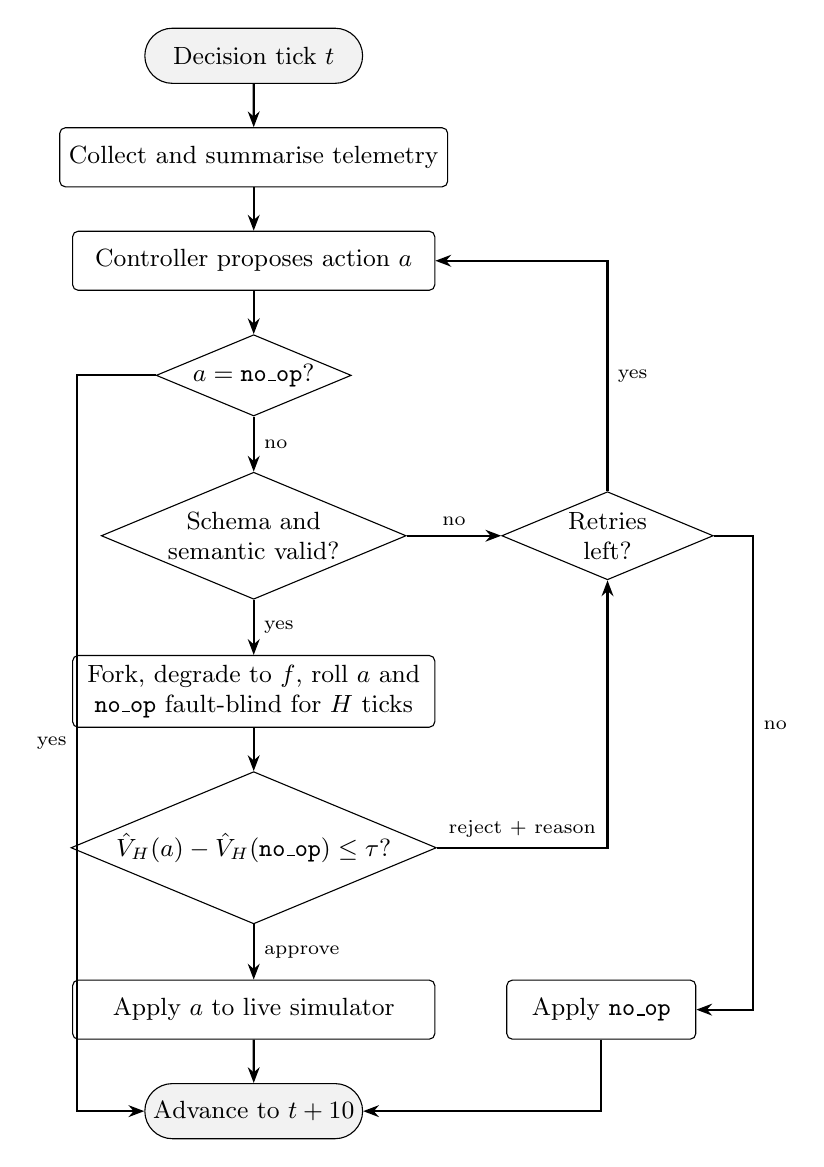
\begin{tikzpicture}[
  node distance=0.55cm,
  proc/.style={draw, rectangle, rounded corners=2pt, align=center, minimum width=4.6cm, minimum height=0.75cm, font=\small},
  dec/.style={draw, diamond, aspect=2.4, align=center, inner sep=1pt, font=\small},
  term/.style={draw, rounded rectangle, align=center, minimum width=3cm, minimum height=0.7cm, font=\small, fill=gray!10},
  arr/.style={-{Stealth[length=2mm]}, thick}
]
\node[term] (s) {Decision tick $t$};
\node[proc, below=of s] (obs) {Collect and summarise telemetry};
\node[proc, below=of obs] (prop) {Controller proposes action $a$};
\node[dec, below=of prop] (noop) {$a = \texttt{no\_op}$?};
\node[dec, below=0.7cm of noop] (valid) {Schema and\\semantic valid?};
\node[proc, below=0.7cm of valid] (twin) {Fork, degrade to $f$, roll $a$ and\\\texttt{no\_op} fault-blind for $H$ ticks};
\node[dec, below=of twin] (gate) {$\hat{V}_H(a) - \hat{V}_H(\texttt{no\_op}) \le \tau$?};
\node[proc, below=0.7cm of gate] (apply) {Apply $a$ to live simulator};
\node[dec, right=1.2cm of valid] (retry) {Retries\\left?};
\node[proc, right=0.9cm of apply, minimum width=2.4cm] (hold) {Apply \texttt{no\_op}};
\node[term, below=of apply] (e) {Advance to $t+10$};
\draw[arr] (s) -- (obs);
\draw[arr] (obs) -- (prop);
\draw[arr] (prop) -- (noop);
\draw[arr] (noop) -- node[right, font=\scriptsize]{no} (valid);
\draw[arr] (valid) -- node[right, font=\scriptsize]{yes} (twin);
\draw[arr] (twin) -- (gate);
\draw[arr] (gate) -- node[right, font=\scriptsize]{approve} (apply);
\draw[arr] (apply) -- (e);
\draw[arr] (valid.east) -- node[above, font=\scriptsize]{no} (retry.west);
\draw[arr] (gate.east) -| node[pos=0.25, above, font=\scriptsize]{reject + reason} (retry.south);
\draw[arr] (retry.north) |- node[pos=0.25, right, font=\scriptsize]{yes} (prop.east);
\draw[arr] (retry.east) -- ++(0.5,0) |- node[pos=0.2, right, font=\scriptsize]{no} (hold.east);
\draw[arr] (noop.west) -- ++(-1.0,0) |- node[pos=0.25, left, font=\scriptsize]{yes} (e.west);
\draw[arr] (hold.south) |- (e.east);
\end{tikzpicture}}
\caption{Flowchart of one gated decision. Rejected or invalid proposals return a reason to the controller, which may retry within its budget; otherwise the system holds.}
\label{fig:flow}
\end{figure}

\begin{algorithm}[t]
\caption{Gated episode with paired counterfactual labelling}
\label{alg:episode}
\begin{algorithmic}[1]
\Require seed $s$, controller $\pi$, gate $g$, fidelity $f$, horizon $H$, tolerance $\tau$, label threshold $\theta$, retry cap $R$
\State $S \gets \textsc{InitSim}(s)$; \; $\mathcal{L} \gets \emptyset$
\For{$t = 0$ \textbf{to} $119$}
  \If{$t \bmod 10 = 0$}
    \State $o \gets \textsc{Summarise}(\textsc{Collect}(S))$; \; $r \gets 0$; \; $\mathit{applied} \gets \textbf{false}$
    \While{$r \le R$ \textbf{and not} $\mathit{applied}$}
      \State $a \gets \pi(o)$
      \State $\Delta \gets \textsc{Label}(S, a, H)$ \Comment{offline, schedule-visible}
      \If{$a = \texttt{no\_op}$} \textbf{break} \EndIf
      \If{$\textsc{Valid}(a, S)$ \textbf{and} $g(S, a, f, H, \tau)$} \State $\textsc{Apply}(S, a)$; \; $\mathit{applied} \gets \textbf{true}$
      \Else \State $o \gets o \cup \{\text{rejection reason}\}$; \; $r \gets r + 1$ \EndIf
      \State $\mathcal{L} \gets \mathcal{L} \cup \{(t, r, a, \Delta, \mathit{applied})\}$
    \EndWhile
  \EndIf
  \State $\textsc{Step}(S)$
\EndFor
\State \Return $V(S)$, $\mathcal{L}$ 
\end{algorithmic}
\end{algorithm}

\subsection{Counterfactual Labels}

For every proposal, including rejected ones and retries, an offline labeller forks the \emph{real} simulator with the fault schedule visible. It rolls out two branches that share exogenous randomness~\cite{crn}: the action followed by \texttt{no\_op}, and \texttt{no\_op} throughout, each for $H = 20$ ticks. The harm delta is
\begin{equation}
D(a) = V_H(a) - V_H(\texttt{no\_op}).
\label{eq:delta}
\end{equation}
$D < 0$ is beneficial, $D = 0$ neutral, and $D > 0$ harmful. For classifier scoring, $a$ is labelled \emph{harmful} if $D(a) > \theta$ with $\theta = 3$. The label is exact \emph{inside the simulator} for the stated state, intervention, continuation policy, and horizon; it is neither a physical-network ground truth nor the action's full closed-loop effect.

\subsection{Evaluation Metrics}

\textbf{Outcome.} The primary outcome is SLO violation-ticks per episode, $V = \sum_{t}\sum_{k} \mathbb{1}[\text{service } k \text{ non-compliant at } t]$; lower is better.

\textbf{Classifier.} With harmful as the positive class, recall $= TP/(TP+FN)$ and $\text{FPR} = FP/(FP+TN)$.

\textbf{Benefit preserved and harm prevented.} Over the non-no-op candidates $\mathcal{C}$ of one arm, with approved set $\mathcal{A}$ and rejected set $\mathcal{R}$,
\begin{equation}
\mathrm{BP} = \frac{\sum_{a \in \mathcal{A}} \max(-D(a),0)}{\sum_{a \in \mathcal{C}} \max(-D(a),0)}, \qquad
\mathrm{HP} = \frac{\sum_{a \in \mathcal{R}} \max(D(a),0)}{\sum_{a \in \mathcal{C}} \max(D(a),0)} .
\label{eq:bphp}
\end{equation}
Reject-all has $\mathrm{BP} = 0$ and $\mathrm{HP} = 1$ by construction. A ratio with a zero denominator is reported as not estimable.

\textbf{Expected advantage over reject-all.} Because reject-all is equivalent to applying \texttt{no\_op} at every decision, the per-seed expected advantage of a gate is approximated by
\begin{equation}
\widehat{\delta}_s = \sum_{a \in \mathcal{A}_s} D(a),
\label{eq:expadv}
\end{equation}
which we compare with the observed paired difference $\delta_s = V_s^{\text{gate}} - V_s^{\text{reject-all}}$.

\textbf{Statistical tests.} Paired differences are zero-inflated, so the primary test is the exact Wilcoxon signed-rank test, with zero differences dropped and the $p$-value obtained by enumerating all $2^m$ sign assignments over $m$ non-tied pairs. Holm correction is applied over 11 comparisons per controller and condition. Paired $t$-intervals and 10,000-resample percentile bootstrap intervals are reported for completeness. With $m$ non-tied pairs the smallest attainable two-sided exact $p$-value is
\begin{equation}
p_{\min}(m) = 2 / 2^{m},
\label{eq:pmin}
\end{equation}
so a comparison that differs on five or fewer of ten seeds cannot reach $p < 0.05$ at any effect size. Seeds required for 80\% power at $\alpha = 0.05$ use $n = \left((z_{1-\alpha/2} + z_{0.8})\,\sigma/|\mu|\right)^2$ and are cross-checked by bootstrap simulation of the Wilcoxon test.

\subsection{Gates Compared}

All gates run with identical seeds, faults, and controller. \emph{Ungated} applies every valid proposal. \emph{Reject-all} blocks every non-no-op proposal and runs no simulation. \emph{Random} blocks at a probability matched to the twin's rejection rate ($p = 0.3$ for rule, $0.747$ for scripted). \emph{Twin@$f$} is Eq.~\eqref{eq:gate} at $f \in \{0.0, 0.6, 1.0\}$. The \emph{schedule-aware} gate applies the same rule on an exact fork that can see the fault schedule; it is not an upper bound on episode performance, because an $H$-tick evaluator can accept actions whose costs fall after $H$. \emph{A0} is the null controller.

\subsection{Implementation and Hardware}

The system is implemented in Python 3.11 with Pydantic schemas, LangGraph, and an OpenAI-compatible client. Telemetry flows sensors $\to$ collector and summariser $\to$ controller $\to$ twin $\to$ an HTTP/1.1 Server-Sent Events server $\to$ a browser dashboard, with typed \texttt{tick}, \texttt{proposal}, \texttt{verdict}, \texttt{applied}, and \texttt{truth} events; identical parameters produce byte-identical streams. The testbed is entirely software: no physical IoT hardware, MQTT broker, or circuit is used, so no circuit diagram or hardware photograph applies. Experiments ran on a single Windows 11 workstation; latency was measured on an isolated host.

% =====================================================================
\section{Experimental Results and Discussion}

\subsection{Experimental Conditions}

Table~\ref{tab:conditions} lists the fixed parameters. Four conditions cross the seed set with the gateway flag. The re-run on seeds 0--9 with the gateway immune reproduces every previously published arm mean exactly.

\begin{table}[t]
\centering
\caption{Experimental conditions.}
\label{tab:conditions}
\footnotesize
\begin{tabular}{@{}p{0.5\columnwidth}p{0.44\columnwidth}@{}}
\toprule
Parameter & Value \\
\midrule
Episode length, decision interval & 120 ticks, every 10 ticks \\
Twin horizon $H$, tolerance $\tau$, label threshold $\theta$ & 20 ticks, 0, 3 violation-ticks \\
Retry cap after rejection & 2 (fallback \texttt{no\_op}) \\
Faults per episode & 3 (start ticks 20--260) \\
Fidelity levels & 0.0, 0.6, 1.0 \\
Condition C1 (primary) & seeds 0--9, gateway immune \\
Condition C2 & seeds 0--9, gateway faultable \\
Condition C3 & gateway-exposed seeds, gateway immune \\
Condition C4 & gateway-exposed seeds, gateway faultable \\
Statistics & exact Wilcoxon, Holm (11 comparisons), $t$-CI, bootstrap CI \\
\bottomrule
\end{tabular}
\end{table}

\subsection{Functional Test Cases and Fault-Handling Mechanism}

Table~\ref{tab:tests} summarises verification. The regression suite grew from 132 to 263 tests during a correctness audit, in which new regression groups initially failed (44 and 6 failures) against the unfixed code, and to 267 with four gateway-flag tests; all pass with warnings treated as errors. Six deliberate mutations of critical code paths were all detected.

\begin{table*}[t]
\centering
\caption{Functional test cases: expected versus actual behaviour.}
\label{tab:tests}
\small
\begin{tabularx}{\textwidth}{@{}p{3.3cm}YYp{1.4cm}@{}}
\toprule
Test case & Condition & Expected result & Actual \\
\midrule
SLO boundary & p95 latency exactly 600.0\,ms; at-risk at 510.0\,ms & Violation flips at 600.0; at-risk flag at 510.0 & Pass \\
Zero-completion tick & Service completes no requests & Tick counted non-compliant, latency \texttt{null} & Pass \\
Malformed commands & Unknown type, missing / extra / mistyped fields & Blocked before actuation & Pass \\
Illegal parameters & NaN, $\pm\infty$, zero or negative throttle; replica cap; memory capacity & Refused with machine-readable reason & Pass \\
Overlapping repairs & Second service-changing action during pending restart / migration & Rejected by shared validation and executor & Pass \\
Route validity & Non-contiguous path, cycle, failed link, wrong endpoint & Rejected & Pass \\
Repair downtime & Restart; five-unit migration & Exactly 3 and 10 unavailable ticks, drops counted & Pass \\
Request conservation & All loss paths & Eq.~\eqref{eq:conservation} holds & Pass \\
Fault composition & Overlapping CPU, link, latency faults; expiry & Contributions add / multiply; only own contribution removed & Pass \\
Gateway crash (flag on) & \texttt{node\_crash} on \texttt{gw0} & Gateway down, all service throughput zero & Pass \\
Twin non-mutation & Gate evaluation on fork & Live state byte-identical & Pass \\
Regression suite & \texttt{pytest -W error} & All pass & 267/267 \\
Mutation check & 6 critical mutations & All detected & 6/6 killed \\
\bottomrule
\end{tabularx}
\end{table*}

\textbf{Fault-handling mechanism.} Faults are handled in four layers. Detection is symptomatic: the collector and summariser expose SLO state, utilisation, memory, and at-risk flags, never the fault type. Proposals then pass schema and semantic validation, which block malformed, infeasible, and conflicting actions before any state is touched. The twin gate rejects actions predicted to worsen violations relative to holding, and returns the reason to the controller. Finally, when retries are exhausted the system holds with \texttt{no\_op} rather than forcing the action, so the worst case of the gate is inaction.

\subsection{Episode Outcomes by Gate}

Table~\ref{tab:perseed} gives per-seed violation-ticks in the primary condition and Figure~\ref{fig:means} the arm means. Reject-all equals A0 on every seed for both controllers: a rejected proposal is retried and ends as a no-op, so reject-all \emph{is} inaction.

\begin{table*}[t]
\centering
\caption{Per-seed SLO violation-ticks, condition C1 (seeds 0--9, gateway immune). Lower is better.}
\label{tab:perseed}
\small
\setlength{\tabcolsep}{4.2pt}
\begin{tabular}{@{}llrrrrrrrrrrr@{}}
\toprule
Controller & Gate & s0 & s1 & s2 & s3 & s4 & s5 & s6 & s7 & s8 & s9 & Mean \\
\midrule
\multirow{8}{*}{Rule}
 & A0 (null)        & 133 & 93 & 125 & 194 & 153 & 101 & 195 & 143 & 120 & 106 & 136.3 \\
 & Ungated          & 133 & 93 & 125 & 194 & 181 & 101 & 170 & 157 & 120 & 110 & 138.4 \\
 & Reject-all       & 133 & 93 & 125 & 194 & 153 & 101 & 195 & 143 & 120 & 106 & 136.3 \\
 & Random $p{=}0.3$ & 133 & 93 & 125 & 194 & 177 & 101 & 170 & 157 & 120 & 123 & 139.3 \\
 & Twin@0.0         & 133 & 93 & 125 & 194 & 170 & 101 & 192 & 143 & 120 & 110 & 138.1 \\
 & Twin@0.6         & 133 & 93 & 125 & 194 & 153 & 101 & 192 & 143 & 120 & 106 & 136.0 \\
 & Twin@1.0         & 133 & 93 & 125 & 194 & 153 & 101 & \textbf{151} & 143 & 120 & 106 & 131.9 \\
 & Schedule-aware   & 133 & 93 & 125 & 194 & 153 & 101 & 151 & 143 & 120 & 106 & 131.9 \\
\midrule
\multirow{6}{*}{Scripted}
 & Ungated            & 152 & 114 & 154 & 202 & 222 & 127 & 248 & 191 & 129 & 122 & 166.1 \\
 & Reject-all         & 133 & 93 & 125 & 194 & 153 & 101 & 195 & 143 & 120 & 106 & 136.3 \\
 & Random $p{=}0.747$ & 145 & 102 & 147 & 208 & 193 & 186 & 198 & 147 & 136 & 135 & 159.7 \\
 & Twin@0.0           & 137 & 113 & 146 & 194 & 169 & 113 & 195 & 143 & 136 & 120 & 146.6 \\
 & Twin@0.6           & 137 & 93 & 130 & 194 & 153 & 101 & 195 & 143 & 120 & 106 & 137.2 \\
 & Twin@1.0           & 133 & 93 & 130 & 194 & 153 & 101 & 195 & 143 & 120 & 106 & 136.8 \\
 & Schedule-aware     & 133 & 93 & 142 & 194 & 140 & 101 & 195 & 143 & 120 & 106 & 136.7 \\
\bottomrule
\end{tabular}
\end{table*}

\begin{figure}[t]
\centering
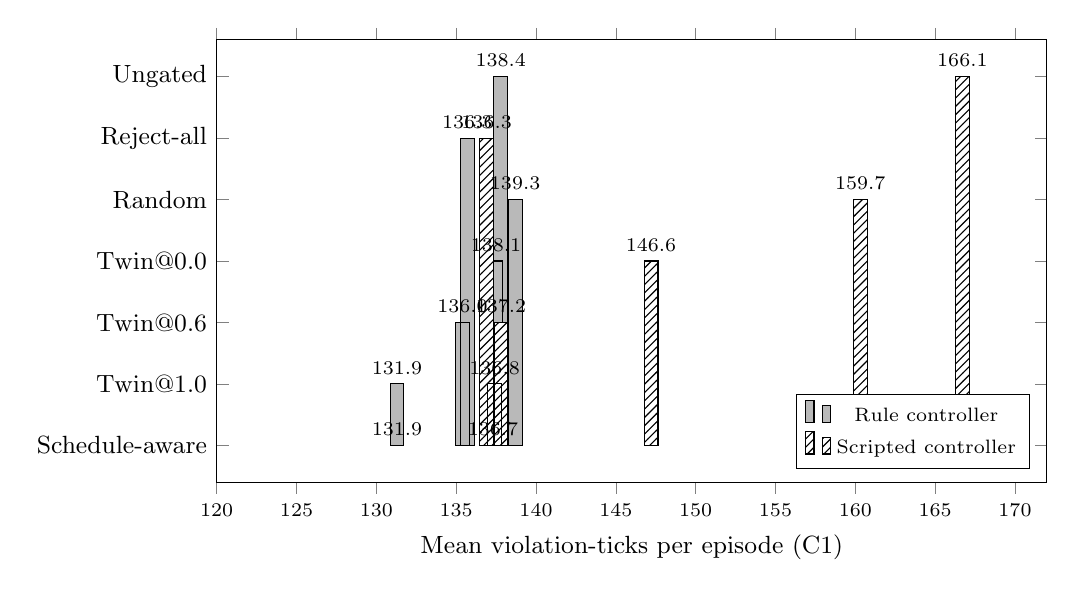
\begin{tikzpicture}
\begin{axis}[
  ybar, width=\columnwidth, height=7.2cm,
  xmin=120, xmax=172, xlabel={Mean violation-ticks per episode (C1)}, xlabel style={font=\small}, x tick label style={font=\scriptsize},
  symbolic y coords={Schedule-aware,Twin@1.0,Twin@0.6,Twin@0.0,Random,Reject-all,Ungated},
  ytick=data, y tick label style={font=\small},
  bar width=5pt, enlarge y limits=0.1,
  legend style={font=\scriptsize, at={(0.98,0.03)}, anchor=south east},
  nodes near coords, nodes near coords style={font=\scriptsize}, point meta=explicit symbolic
]
\addplot[fill=gray!55, draw=black] coordinates {
  (138.4,Ungated) [138.4] (136.3,Reject-all) [136.3] (139.3,Random) [139.3]
  (138.1,Twin@0.0) [138.1] (136.0,Twin@0.6) [136.0] (131.9,Twin@1.0) [131.9] (131.9,Schedule-aware) [131.9]};
\addplot[fill=white, draw=black, postaction={pattern=north east lines}] coordinates {
  (166.1,Ungated) [166.1] (136.3,Reject-all) [136.3] (159.7,Random) [159.7]
  (146.6,Twin@0.0) [146.6] (137.2,Twin@0.6) [137.2] (136.8,Twin@1.0) [136.8] (136.7,Schedule-aware) [136.7]};
\legend{Rule controller, Scripted controller}
\end{axis}
\end{tikzpicture}
\caption{Mean violation-ticks by gate in condition C1. Means hide that differences between gates are concentrated in one to three seeds (Table~\ref{tab:perseed}).}
\label{fig:means}
\end{figure}

On means alone, the full-fidelity twin appears to help the rule controller by 4.4 violation-ticks relative to reject-all and to match the schedule-aware gate, while for the scripted controller reject-all (136.3) is marginally better than the twin (136.8). Table~\ref{tab:paired} shows that these differences are not established.

\begin{table*}[t]
\centering
\caption{Paired comparisons in condition C1 (first arm minus second; negative favours the first arm). B/T/W: seeds better / tied / worse. $p$: exact Wilcoxon; Holm over 11 comparisons.}
\label{tab:paired}
\small
\setlength{\tabcolsep}{4pt}
\begin{tabular}{@{}llrrcccc@{}}
\toprule
Controller & Comparison & Mean & SD & 95\% $t$-CI & B/T/W & $p$ & $p_{\text{Holm}}$ \\
\midrule
\multirow{5}{*}{Rule}
 & Twin@1.0 $-$ reject-all & $-4.40$ & 13.91 & $[-14.35, +5.55]$ & 1/9/0 & 1.000 & 1.000 \\
 & Twin@1.0 $-$ ungated    & $-6.50$ & 10.19 & $[-13.79, +0.79]$ & 4/6/0 & 0.125 & 1.000 \\
 & Reject-all $-$ ungated  & $-2.10$ & 13.24 & $[-11.57, +7.37]$ & 3/6/1 & 0.625 & 1.000 \\
 & Twin@1.0 $-$ twin@0.0   & $-6.20$ & 13.34 & $[-15.74, +3.34]$ & 3/7/0 & 0.250 & 1.000 \\
 & Schedule-aware $-$ twin@1.0 & 0.00 & 0.00 & $[0, 0]$ & 0/10/0 & -- & -- \\
\midrule
\multirow{6}{*}{Scripted}
 & Twin@1.0 $-$ reject-all & $+0.50$ & 1.58 & $[-0.63, +1.63]$ & 0/9/1 & 1.000 & 1.000 \\
 & \textbf{Twin@1.0 $-$ ungated} & $\mathbf{-29.30}$ & 20.40 & $[-43.89, -14.71]$ & 10/0/0 & 0.0020 & \textbf{0.0215} \\
 & \textbf{Reject-all $-$ ungated} & $\mathbf{-29.80}$ & 20.31 & $[-44.33, -15.27]$ & 10/0/0 & 0.0020 & \textbf{0.0215} \\
 & Twin@0.0 $-$ reject-all & $+10.30$ & 8.49 & $[+4.23, +16.37]$ & 0/3/7 & 0.0156 & 0.125 \\
 & Twin@1.0 $-$ twin@0.0   & $-9.80$ & 7.91 & $[-15.46, -4.14]$ & 7/3/0 & 0.0156 & 0.125 \\
 & Schedule-aware $-$ twin@1.0 & $-0.10$ & 5.90 & $[-4.32, +4.12]$ & 1/8/1 & 1.000 & 1.000 \\
\bottomrule
\end{tabular}
\end{table*}

\textbf{Discussion.} For the rule controller, none of the 11 comparisons is distinguishable from noise at ten seeds. The twin@1.0 advantage over reject-all comes from seed 6 alone (per-seed differences $[0,0,0,0,0,0,-44,0,0,0]$), so by Eq.~\eqref{eq:pmin} no rank test could reach significance. On that seed the twin approved a \texttt{restart\_service} during a memory leak ($D = -29$) that reject-all blocked. Even the twin versus ungated comparison, better on four seeds and worse on none, has a minimum attainable $p$ of 0.125. For the scripted controller, the only results that survive Holm correction are that the ungated controller is harmful and that \emph{any} blocking gate removes that harm, by about 29--30 violation-ticks on all ten seeds. The twin cannot be told apart from reject-all, and its point estimate is slightly worse. The fidelity effect (twin@1.0 better than twin@0.0 by 9.8) is significant only before correction.

\subsection{The Gate as a Local Classifier}

At $f = 1.0$ the twin achieves 96.1\% recall at 4.07\% FPR on the scripted controller's proposals and 100\% recall at 0.83\% FPR on the rule controller's. Table~\ref{tab:bphp} reports benefit preserved and harm prevented (Eq.~\eqref{eq:bphp}) on each arm's own candidates. For the rule controller, the full-fidelity twin matches reject-all on harm and keeps all of the benefit: as a filter it is strictly better than reject-all and identical to the schedule-aware gate. For the scripted controller it leaks 10 violation-ticks of harm to keep 26 of benefit. At $f = 0.0$ the scripted controller's leaked harm (98) exceeds its preserved benefit (60), so the degraded twin is expected to do worse than reject-all, consistent with the observed $+10.3$.

\begin{table*}[t]
\centering
\caption{Benefit preserved (BP) and harm prevented (HP) on each arm's own non-no-op candidates, condition C1. Values in violation-ticks.}
\label{tab:bphp}
\small
\setlength{\tabcolsep}{4.5pt}
\begin{tabular}{@{}llrcccr@{}}
\toprule
Controller & Gate & Cand. & Benefit appr./avail. & BP & HP & Net $\sum D$ approved \\
\midrule
\multirow{5}{*}{Rule}
 & Reject-all     & 13 & 0 / 35  & 0.000 & 1.000 & 0 \\
 & Twin@0.0       & 14 & 21 / 50 & 0.420 & 0.714 & $-3$ \\
 & Twin@0.6       & 14 & 15 / 44 & 0.341 & 1.000 & $-15$ \\
 & \textbf{Twin@1.0} & 15 & 44 / 44 & \textbf{1.000} & \textbf{1.000} & $-44$ \\
 & Schedule-aware & 15 & 44 / 44 & 1.000 & 1.000 & $-44$ \\
\midrule
\multirow{5}{*}{Scripted}
 & Reject-all     & 72 & 0 / 2    & 0.000 & 1.000 & 0 \\
 & Twin@0.0       & 76 & 60 / 100 & 0.600 & 0.690 & $+38$ \\
 & Twin@0.6       & 72 & 20 / 22  & 0.909 & 0.961 & $-4$ \\
 & \textbf{Twin@1.0} & 73 & 26 / 28 & \textbf{0.929} & \textbf{0.976} & $-16$ \\
 & Schedule-aware & 72 & 18 / 18  & 1.000 & 1.000 & $-18$ \\
\bottomrule
\end{tabular}
\end{table*}

\subsection{Why an Accurate Filter Yields a Null: Candidate Composition}

Table~\ref{tab:composition} shows the composition of proposals. The rule controller proposes a no-op 88.3\% of the time, about 1.5 candidates per episode per arm. Thirty percent of its non-no-op candidates are beneficial, but de-duplicated across arms they amount to 9 distinct beneficial decisions, and the single seed-6 restart accounts for 54\% of its pooled available benefit. The scripted controller's only action, \texttt{scale\_service}, is harmful 63\% of the time, with beneficial and harmful scale-ups of similar magnitude (median 6--8 ticks) but harmful ones 2.4--3.6 times more numerous.

\begin{table*}[t]
\centering
\caption{Candidate composition, condition C1, pooled over all arms. $D$ from Eq.~\eqref{eq:delta}.}
\label{tab:composition}
\small
\setlength{\tabcolsep}{4pt}
\begin{tabular}{@{}llrrrrrr@{}}
\toprule
Controller & Action & Cand. & Beneficial & Neutral & Harmful & $\sum |D|$, $D<0$ & $\sum D$, $D>0$ \\
\midrule
Rule & \texttt{restart\_service} & 8 & 8 (100\%) & 0 & 0 & 202 & 0 \\
Rule & \texttt{scale\_service} & 111 & 28 (25\%) & 16 & 67 (60\%) & 171 & 467 \\
\textbf{Rule} & \textbf{all} & \textbf{119} & \textbf{36 (30\%)} & 16 & \textbf{67 (56\%)} & \textbf{373} & \textbf{467} \\
Scripted & \texttt{scale\_service} & 610 & 106 (17\%) & 119 & 385 (63\%) & 721 & 2,676 \\
\bottomrule
\end{tabular}
\end{table*}

What matters is the benefit available on the gated trajectories. On the twin@1.0 trajectory the rule controller offered 44 violation-ticks of benefit over ten episodes, all in seed 6, and reject-all discarded only 35. The scripted controller offered 28 ticks of benefit against 420 of harm, and on the reject-all trajectory only 2 ticks of benefit existed in ten episodes. Gating also changes the candidate population: ungated, the scripted controller faces 26 beneficial candidates, but behind a gate only 1--4 remain, because blocked scale-ups leave services degraded and later scale-ups from persistently degraded states are rarely beneficial. A gate cannot beat reject-all by more than reject-all throws away.

\subsection{Expected versus Actual Results}

Table~\ref{tab:expected} compares the expected advantage of Eq.~\eqref{eq:expadv} with the observed paired difference. For the rule controller in the primary condition, the prediction is exact. Even a perfect gate would gain at most 3.5--4.4 ticks per seed against a paired SD of 13.9, which gives about 17\% power at ten seeds and requires 79--125 seeds under a normal approximation. For the scripted controller, no gate could gain more than 0.2 ticks per seed over reject-all, which would require about 491 seeds. However, the per-decision arithmetic gets the scripted controller's \emph{sign} wrong in all four conditions and underestimates the rule controller's migration effects 3--6 times on gateway-exposed seeds. On scripted seed 2 the twin approved four scale-ups with $D = +2, +4, -13, -6$ (net $-13$), yet the episode ended 5 ticks worse than reject-all. Twenty-tick counterfactuals with a no-op continuation do not add up to closed-loop episode effects.

\begin{table}[t]
\centering
\caption{Expected (Eq.~\eqref{eq:expadv}) versus actual twin@1.0 $-$ reject-all, per-seed mean violation-ticks.}
\label{tab:expected}
\footnotesize
\setlength{\tabcolsep}{3pt}
\begin{tabular}{@{}llrrl@{}}
\toprule
Condition & Controller & Expected & Actual & Agreement \\
\midrule
C1 seeds 0--9, immune       & Rule     & $-4.4$ & $-4.4$ & exact \\
C1 seeds 0--9, immune       & Scripted & $-1.6$ & $+0.5$ & wrong sign \\
C2 seeds 0--9, faultable    & Rule     & $-2.9$ & $-4.1$ & 1.4$\times$ \\
C2 seeds 0--9, faultable    & Scripted & $-1.3$ & $+0.5$ & wrong sign \\
C3 exposed seeds, immune    & Rule     & $-0.7$ & $-2.3$ & 3.3$\times$ \\
C3 exposed seeds, immune    & Scripted & $-1.0$ & $+0.7$ & wrong sign \\
C4 exposed seeds, faultable & Rule     & $-0.8$ & $-4.8$ & 6.0$\times$ \\
C4 exposed seeds, faultable & Scripted & $-1.0$ & $+3.3$ & wrong sign \\
\bottomrule
\end{tabular}
\end{table}

\subsection{Gateway Ablation}

Every device attaches to the gateway, and by default node faults never target it, which could make it a fault-immune refuge. Across all four conditions, two controllers, eight gates, and about 9,200 proposals, \emph{no} proposal migrated a service to the gateway: the rule controller only targets edge nodes, and the scripted controller never migrates. The gateway's share of migration benefit is therefore 0\%. Table~\ref{tab:gateway} shows that the twin's advantage over reject-all is no clearer when the gateway can fail. Enabling the flag also re-targets some edge faults (the target pool changes), so condition C2 is a different fault placement rather than a test of gateway failure; C3 and C4 are the genuine test. Gateway faults are severe, raising A0 from 143.7 to 213.5 mean violation-ticks.

\begin{table*}[t]
\centering
\caption{Twin@1.0 $-$ reject-all under the four gateway conditions.}
\label{tab:gateway}
\small
\setlength{\tabcolsep}{4pt}
\begin{tabular}{@{}lllrrcc@{}}
\toprule
Controller & Condition & Per-seed differences & Twin@1.0 & Reject-all & Mean [95\% $t$-CI] & $p$ \\
\midrule
\multirow{4}{*}{Rule}
 & C1 & one seed: $-44$ & 131.9 & 136.3 & $-4.40$ $[-14.35, +5.55]$ & 1.000 \\
 & C2 & one seed: $-41$ & 128.1 & 132.2 & $-4.10$ $[-13.37, +5.17]$ & 1.000 \\
 & C3 & one seed: $-23$ & 141.4 & 143.7 & $-2.30$ $[-7.50, +2.90]$ & 1.000 \\
 & C4 & one seed: $-48$ & 208.7 & 213.5 & $-4.80$ $[-15.66, +6.06]$ & 1.000 \\
\midrule
\multirow{4}{*}{Scripted}
 & C1 & one seed: $+5$ & 136.8 & 136.3 & $+0.50$ $[-0.63, +1.63]$ & 1.000 \\
 & C2 & one seed: $+5$ & 132.7 & 132.2 & $+0.50$ $[-0.63, +1.63]$ & 1.000 \\
 & C3 & one seed: $+7$ & 144.4 & 143.7 & $+0.70$ $[-0.88, +2.28]$ & 1.000 \\
 & C4 & two seeds: $+20, +13$ & 216.8 & 213.5 & $+3.30$ $[-1.81, +8.41]$ & 0.500 \\
\bottomrule
\end{tabular}
\end{table*}

On gateway-exposed seeds with the gateway immune, twin@0.6 (138.9) outperforms twin@1.0 (141.4) for the rule controller, so the fidelity ordering is not stable once migrations occur, consistent with the non-monotone fidelity effects reported by Su \emph{et al.}~\cite{fidelityam}.

\subsection{Opportunity Gap}

To test whether useful repairs exist at all, a privileged diagnostic enumerator with exact state, the fault schedule, and cloned random streams scores every valid candidate. No controller or gate imports it. Table~\ref{tab:opp} gives single-fault results (seed 0, 80-tick faults, 60-tick horizon). Every fault type has a beneficial candidate, but for four of the six the best move migrates the affected service to the gateway, and excluding the gateway roughly halves the benefit; the gateway asymmetry therefore does affect this analysis. Over seeds 0--1 (16 decision points, 40-tick horizon), a beneficial action existed at all 16 points, worth 130 violation-ticks in total, while the rule controller held at all 16. Enumerator advice also does not compose: migrating one service to the gateway reduces violations (seed 0: 44 $\to$ 28), but migrating all six saturates it and yields the maximum of 360.

\begin{table}[t]
\centering
\caption{Privileged candidate search (seed 0, single 80-tick fault, 60-tick horizon). Service violation-ticks.}
\label{tab:opp}
\footnotesize
\begin{tabular}{@{}lcccc@{}}
\toprule
Fault & Hold & Best & Best w/o gw & Best non-migr. \\
\midrule
CPU saturation   & 145 & 95 & 117 & 144 \\
Node crash       & 145 & 95 & 115 & 144 \\
Link degradation & 145 & 95 & 115 & 144 \\
Link failure     & 145 & 95 & 115 & 144 \\
Memory leak      & 107 & 55 & 55  & 55  \\
Traffic surge    & 94  & 79 & 85  & 85  \\
\bottomrule
\end{tabular}
\end{table}

\subsection{Performance Comparison: Cost of the Gate}

Table~\ref{tab:latency} reports per-stage latency. These timings were measured on the pre-correction simulator and have not yet been re-measured; the simulator changes affect semantics, not the forking mechanism, so we expect the order of magnitude to hold. The gate raises decision latency from about 0.1\,ms to about 81\,ms, which is small relative to the decision interval but grows linearly with horizon and topology size. CPU time for a 10-seed run rose from 90.4\,s (rule, ungated) to 166.8\,s (rule, twin-gated). On loopback, the SSE chain showed a 2.60\,ms median request latency and 3.2\,ms to first event.

\begin{table}[t]
\centering
\caption{Per-stage latency (isolated host; pre-correction simulator).}
\label{tab:latency}
\footnotesize
\begin{tabular}{@{}p{0.52\columnwidth}p{0.42\columnwidth}@{}}
\toprule
Stage & Median latency \\
\midrule
Simulator tick & 1.77\,ms \\
Collect + summarise + rule decision + validation & $\sim$0.1\,ms \\
State fork & 0.91\,ms \\
Twin validation, $H = 20$ (across fidelities) & 73.8--82.1\,ms (worst p95 100.4\,ms) \\
Horizon sweep twin cost, $H = 5 / 10 / 20 / 40$ & 29.0 / 42.0 / 75.8 / 142.6\,ms \\
\bottomrule
\end{tabular}
\end{table}

\subsection{Summary of Findings}

(i) An accurate local filter is not sufficient for a detectable outcome benefit: at full fidelity the twin prevents essentially all harm and preserves essentially all benefit, but the benefit reachable on gated trajectories is tiny and concentrated in one to three seeds. (ii) Reject-all is a necessary control: without it, the scripted controller's 29.3-tick improvement over ungated would be misattributed to prediction, when reject-all achieves 29.8. (iii) The binding constraint is the proposer, not the gate: real repairs exist at every sampled decision point, but the controllers rarely propose them. (iv) Per-decision counterfactual sums are a poor substitute for closed-loop measurement.

% =====================================================================
\section{Limitations and Future Work}
\label{sec:limits}

\textbf{Limitations.}
\begin{itemize}
  \item \emph{Synthetic testbed.} All results come from a 17-node simulator with no physical hardware and a loopback transport. No numerical comparison with systems evaluated on realistic replicas, such as Aether~\cite{aether}, is meaningful.
  \item \emph{No real LLM arm.} The one arm driven by a real model (cached) emitted \texttt{no\_op} in about 97\% of decisions, leaving an almost empty confusion matrix. All results for aggressive agents come from a scripted stub, which always proposed \texttt{no\_op} on retry, so repair by re-prompting is untested.
  \item \emph{Statistical power.} Ten seeds cannot detect effects carried by one seed. The estimate that 79--125 seeds would be needed assumes that about 10\% of episodes contain a decision where selective approval matters, and that rate rests on a single event (95\% Clopper--Pearson interval 0.25\%--44.5\%).
  \item \emph{Shared code between twin and labeller.} Both are the same simulator in different fault modes, so twin errors are structurally correlated with the labels.
  \item \emph{Label definition.} Labels use a single rollout, a \texttt{no\_op} continuation, and a finite horizon; with $\tau = 0$ and $\theta = 3$, actions with true harm of 1--3 ticks count as false positives even when the twin is directionally correct.
  \item \emph{Gateway flag design.} Enabling \texttt{gateway\_faultable} changes how random draws map to targets, so it is a different fault distribution rather than a strict superset of the default.
  \item \emph{Staleness approximation and pre-correction timings.} The staleness axis scales current degradation toward baseline instead of replaying a stored past state, and latency and horizon timings remain to be re-measured on the corrected simulator.
\end{itemize}

\textbf{Future work.}
\begin{enumerate}
  \item Design workloads in which most episodes contain a decision with substantial repair benefit (tens of violation-ticks per episode), rather than adding seeds to the current workload.
  \item Build a decisive proposer, including a working LLM arm, that regularly offers restarts for leaks and migrations for sustained node faults, and measure retry-based repair.
  \item Draw gateway faults as a separate Bernoulli event so that edge targeting is unchanged, and re-run the opportunity-gap analysis with a faultable gateway.
  \item Re-score classifiers on a frozen corpus of identical (state, candidate) pairs, sweep $\tau$ for precision--recall curves, and re-measure horizon and latency.
  \item Model fault-arrival uncertainty with legitimately available information, such as disturbance ensembles~\cite{robustmps,pomcp}, without supplying the hidden schedule.
  \item Add an independently implemented twin (a queueing approximation or learned surrogate), an MQTT transport, and larger topologies.
\end{enumerate}

% =====================================================================
\section{Conclusion}

Twin-in-the-Loop is a deterministic testbed for measuring what an imperfect digital twin contributes when it vets autonomous edge-network repairs. It labels every proposal with a paired counterfactual, degrades the twin along five controllable axes, and compares it with reject-all, random, and schedule-aware gates under exact paired statistics. The central finding is a dissociation: at full fidelity the twin is a near-perfect local filter, preserving 100\% and 92.9\% of available benefit and preventing 100\% and 97.6\% of available harm for the rule and scripted controllers, yet it cannot be distinguished from reject-all at the episode level. The only effects that survive multiplicity correction are that the scripted controller is harmful ungated and that any blocking gate removes about 30 violation-ticks of that harm. Candidate composition explains the null: reject-all discards only 35 and 2 violation-ticks of benefit across ten episodes, so even a perfect gate would be underpowered, and an unfaultable-gateway ablation rules out a topology artifact. Evaluations of twin-gated agents should therefore report a reject-all control, per-seed distributions, and the benefit actually available to the gate, and should pair twin gates with proposers that offer real repairs.

% =====================================================================
\section*{CRediT authorship contribution statement}

\textbf{Nitin Kumar Pandey, Ayush Raj, Abhay Mahantesh Zalaki, Guneet Kaur Arora:} Conceptualization, Methodology, Software, Validation, Formal analysis, Investigation, Data curation, Visualization, Writing -- original draft.
\textbf{Syamasudha Veeragandham:} Conceptualization, Supervision, Project administration, Writing -- review \& editing.

\section*{Funding Statement}

The authors declare that no funding, grants, or external support were received during the development of this work.

\section*{Declaration of competing interest}

The authors declare that they have no known competing financial interests or personal relationships that could have appeared to influence the work reported in this paper.

\section*{Data Availability}

No external data were used. All data were generated by the simulator described in this paper and can be regenerated deterministically from the stated seeds. The source code, experiment scripts, per-seed statistics, and labelled proposal records are available from the corresponding author on reasonable request.

% =====================================================================
% References are numbered in order of first citation.
\begin{thebibliography}{00}

\bibitem{microremed} ``MicroRemed: Benchmarking LLMs in microservices remediation,'' arXiv:2511.01166, 2025.

\bibitem{nika} ``A network arena for benchmarking AI agents on network troubleshooting,'' arXiv:2512.16381, 2025.

\bibitem{netagentbench} ``NetAgentBench: A state-centric benchmark for evaluating agentic network configuration,'' arXiv:2604.09678, 2026.

\bibitem{aether} ``Aether: Network validation using agentic AI and digital twin,'' arXiv:2604.18233, 2026.

\bibitem{processplant} ``Leveraging LLM agents and digital twins for fault handling in process plants,'' in \emph{Proc. IEEE Int. Conf. Emerging Technologies and Factory Automation (ETFA)}, 2025, arXiv:2505.02076.

\bibitem{simplex} M.~Rivera \emph{et al.}, ``An architectural description of the Simplex architecture,'' Software Engineering Institute, Carnegie Mellon University, Tech. Rep. CMU/SEI-96-TR-006, 1996.

\bibitem{wabersich} K.~P. Wabersich and M.~N. Zeilinger, ``A predictive safety filter for learning-based control of constrained nonlinear dynamical systems,'' \emph{Automatica}, vol.~129, 109597, 2021, doi:10.1016/j.automatica.2021.109597.

\bibitem{mps} O.~Bastani, ``Safe reinforcement learning with nonlinear dynamics via model predictive shielding,'' arXiv:1905.10691, 2019.

\bibitem{rawlings} J.~B. Rawlings, D.~Q. Mayne, and M.~M. Diehl, \emph{Model Predictive Control: Theory, Computation, and Design}, 2nd ed. Madison, WI, USA: Nob Hill Publishing, 2017.

\bibitem{netinjectbench} ``NetInjectBench: Benchmarking indirect prompt injection in tool-using large language model agents for network operations,'' arXiv:2607.10490, 2026.

\bibitem{agentdojo} E.~Debenedetti, J.~Zhang, M.~Balunovi\'c, L.~Beurer-Kellner, M.~Fischer, and F.~Tram\`er, ``AgentDojo: A dynamic environment to evaluate prompt injection attacks and defenses for LLM agents,'' in \emph{Proc. NeurIPS Datasets and Benchmarks Track}, 2024.

\bibitem{fidelityam} C.~Su, B.~Hicks, and A.~Nassehi, ``Investigating the influence of fidelity on the capability of a digital twin to detect material extrusion failures,'' \emph{Journal of Intelligent Manufacturing}, vol.~35, pp.~2263--2276, 2024, doi:10.1007/s10845-023-02144-x.

\bibitem{mbpo} M.~Janner, J.~Fu, M.~Zhang, and S.~Levine, ``When to trust your model: Model-based policy optimization,'' in \emph{Proc. NeurIPS}, 2019.

\bibitem{sampath} M.~Sampath, R.~Sengupta, S.~Lafortune, K.~Sinnamohideen, and D.~Teneketzis, ``Diagnosability of discrete-event systems,'' \emph{IEEE Transactions on Automatic Control}, vol.~40, no.~9, pp.~1555--1575, 1995, doi:10.1109/9.412626.

\bibitem{pomcp} D.~Silver and J.~Veness, ``Monte-Carlo planning in large POMDPs,'' in \emph{Proc. NeurIPS}, 2010.

\bibitem{k8scontroller} The Kubernetes Authors, ``Controllers,'' Kubernetes documentation. [Online]. Available: https://kubernetes.io/docs/concepts/architecture/controller/

\bibitem{k8shpa} The Kubernetes Authors, ``Horizontal Pod Autoscaling,'' Kubernetes documentation. [Online]. Available: https://kubernetes.io/docs/concepts/workloads/autoscaling/horizontal-pod-autoscale/

\bibitem{sre_cascade} B.~Beyer, C.~Jones, J.~Petoff, and N.~R. Murphy, Eds., ``Addressing cascading failures,'' in \emph{Site Reliability Engineering: How Google Runs Production Systems}. Sebastopol, CA, USA: O'Reilly Media, 2016.

\bibitem{budgetaware} Liu \emph{et al.}, ``Budget-aware tool use enables effective agent scaling,'' arXiv:2511.17006, 2025.

\bibitem{langgraph} LangChain, ``Graph API: Recursion limit,'' LangGraph documentation. [Online]. Available: https://docs.langchain.com/oss/python/langgraph/graph-api

\bibitem{crn} W.-N. Yang and B.~L. Nelson, ``Using common random numbers and control variates in multiple-comparison procedures,'' \emph{Operations Research}, vol.~39, no.~4, pp.~583--591, 1991, doi:10.1287/opre.39.4.583.

\bibitem{yadav} Yadav \emph{et al.}, ``Using common random numbers for simulation-based planning with rollouts,'' in \emph{Proc. Reinforcement Learning Conference (RLC)}, 2026.

\bibitem{rulebasedshield} Shperberg \emph{et al.}, ``A rule-based shield: Accumulating safety rules from catastrophic action effects,'' in \emph{Proc. Conference on Lifelong Learning Agents (CoLLAs)}, PMLR vol.~199, 2022.

\bibitem{saferlsurvey} ``A survey of safe reinforcement learning and constrained MDPs: A technical survey on single-agent and multi-agent safety,'' arXiv:2505.17342, 2025.

\bibitem{slbench} ``SLBench,'' arXiv:2607.09016, 2026.

\bibitem{robustmps} S.~Li and O.~Bastani, ``Robust model predictive shielding for safe reinforcement learning with stochastic dynamics,'' arXiv:1910.10885, 2019.

\bibitem{vaml} A.-m. Farahmand, ``Iterative value-aware model learning,'' in \emph{Proc. NeurIPS}, 2018.

\bibitem{cabasino} M.~P. Cabasino, A.~Giua, and C.~Seatzu, ``Diagnosability of discrete-event systems using labeled Petri nets,'' \emph{IEEE Transactions on Automation Science and Engineering}, 2014, doi:10.1109/TASE.2013.2289360.

\bibitem{sre_monitoring} B.~Beyer, C.~Jones, J.~Petoff, and N.~R. Murphy, Eds., ``Monitoring distributed systems,'' in \emph{Site Reliability Engineering: How Google Runs Production Systems}. Sebastopol, CA, USA: O'Reilly Media, 2016.

\end{thebibliography}

\end{document}
